\chapter{Background}

\section{Spectral Clustering}

It is convenient to set a little context, in order to appreciate
better what is the operation that this thesis tries to optimize; for
this we enter a bit into the Spectral Clustering world. In such
context the Laplacian Matrix and its second smallest eigenvector
\footnote{This is an abuse of the language of course, when
we say the smallest or biggest eigenvector or eigenpair, we actually refer to
the property of the associated eigenvalue.}
(Fiedler Vector) will emerge; and it will become clearer why computing
an eigenvector can serve data clustering. The original merit of
finding the value of the Fiedler Vector goes to Fiedler
\cite{fiedler73}, considered the father of Algebraic Graph Theory; and
the stuff we briefly discuss on this chapter could be considered part
of one its branches, Spectral Graph Theory (\cite{brouwer12}). In
practical terms, the material exposed here comes mainly from the
standard introductory book to Spectral Clustering by Luxburg \cite{luxburg07},
and from the excellent lecture that Prof. Gao gives about the topic on
its Data Mining Course at the University of Buffalo \cite{gao13}.

\subsection{Minimal Bi-Partitional RatioCut}

If you are doing Data Clustering, you encode your applications' data
into vectors $\vec{x} \in \R{n}$; but if you are aiming to do Spectral
Clustering you will also need to build an auxiliary graph. This is
because in Spectral Clustering, the operation of computing clusters is
reduced to that of computing graph partitions. To do that, you need to
label your encoded data (vectors) as nodes in an undirected weighted graph $G =
(V,W)$; where the edges between them will contain as weights the value 
of a similarity function defined for the given problem. \\

The work of this thesis lies around the basic operation of
bi-partitioning such graph (removing certain edges such that we
disconnect the vertices set). This is to be done in such way that the
\emph{cut} function $\left(\func{cut}(A,B) = \sum\limits_{\tiny{i \in A
    \ds{,} j \in B}} w_{ij}\right)$ is minimized. This will bring as result
two partitions with quite similar nodes (according to the similarity
function defined); and then, they could be thought as clusters. The
following figure (adapted from \cite{gao13}) illustrates the
operation:

\begin{figure}[H]
  \label{min-bip-cut}
  \centering
  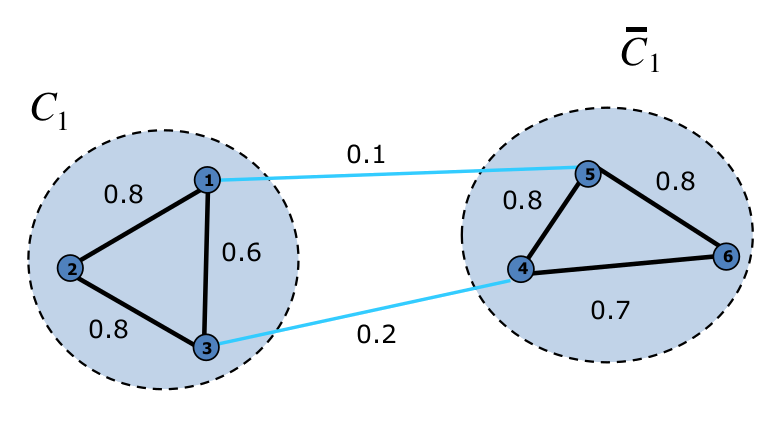
\includegraphics[width=10cm,height=5.5cm]{min-bip-cut-doc}
\end{figure}

The sky blue edges are the minimal \emph{cut} for this example; resulting
in two partitions $C_1$ and $\stcomp{C_1}$. While there is more than
one way of formalizing this problem, the way we care about is the one
using the \emph{RatioCut} function (Minimal Bi-Partitional RatioCut Problem);
which favors the solutions which have partitions of roughly
the same size: 

\begin{equation*}
  \min\limits_{\tiny{C_1 \ds{\subset} V}} \ds{}
  \underbrace{      
    \frac{1}{2}
    \left[
      \dfrac{\func{cut}(C_1,\stcomp{C_1})}{\abs{C_1}} +
      \dfrac{\func{cut}(\stcomp{C_1},C_1)}{\abs{\stcomp{C_1}}}
      \right]
  }_{\func{RatioCut(C_1,\stcomp{C_1})}}
  \ds{\suchthat}
  \func{cut}(A,B) = \sum\limits_{\tiny{i \in A \ds{,} j \in B}} w_{ij}
\end{equation*}
\joinbelow{1cm}

Asking for the partitions to have similar sizes avoids the non
interesting solutions which include singleton partitions; but it also
has the side effect of making the optimization problem NP-Hard. This
is where Spectral Clustering comes to rescue us; by using Linear
Algebra techniques, it can approximate the solutions to the problem
above.

\subsection{The Laplacian and its Fiedler Vector}
The details can be consulted at \cite{luxburg07} or
\cite{gao13}, but it turns out that if we define the (unnormalized)
Laplacian Matrix as $L = D - W$ (where $D$ is the diagonal containing
the nodes' degrees and $W$ is the weights matrix of the graph); then
the Minimal Bi-Partitional RatioCut Problem reduces to that of minimizing the
Rayleigh-Quotient Function:

\begin{equation*}
\min\limits_{C_1 \ds{\subset} V} \func{RatioCut}(C1,\stcomp{C1})
\ds{\ds{\equiv}}
\min\limits_{\vec{f} \in \R{n}}
  \underbrace{
    \left(\dfrac{\trans{\vec{f}} L \ds{\vec{f}}}{\trans{\vec{f}} \vec{f}}\right)
  }_{\text{Rayleigh-Quotient}}    
\ds{\suchthat}
\vec{f} \in \R{n} \ds{\land} \vec{f} \bot \vec{1}
\end{equation*}
\joinbelow{1cm}

The solution given by the vector $\vec{f}$ is an approximation, and it acts
as an indicator function; each one of its cells represents one node in
the graph, and its sign tells whether the associated node belongs to
partition $C_1$ or its complement $\stcomp{C_1}$. The property of $f$
being orthogonal to the vector $\vec{1}$ is a consequence of the
Laplacian matrix ($L$) and the Rayleigh-Quotient function
properties. \\

The advantage of having formulated the problem in terms of the
Rayleigh-Quotient function, allows us to use the immense arsenal that
Linear Algebra has at our disposal. This step is usually skip in
literature, but here we include a more explicit argument; the concrete
theorem that clearly gives a solution to the above problem is the
Courant-Fischer Theorem (specialized for the case of the second
smallest eigenvalue of a real-symmetric matrix $A$):

\begin{equation*}
\lambda_2(A) =
\max\limits_{\func{dim}(U) = n-1}
\left[
\min\limits_{\vec{x} \in U \ds{\land} \norm{\vec{x}} \ne 0}
\left(  
\dfrac{\trans{\vec{x}} A \ds{\vec{x}}}{\trans{\vec{x}} \vec{x}}
\right)
\right]
\end{equation*}
\joinbelow{1cm}

The above result basically tells us that, if we were able to navigate
throughout all the subspaces of dimension $n-1$ (where $n$ is the
dimension of the Laplacian matrix), then we would know that the answer
to our problem is the eigenvector associated to the second-smallest
eigenvalue of the Laplacian (called Fiedler Vector). The only obstacle
in applying this mighty result, is the non practical task of iterating
over an infinite number of subspaces; but the previously stated
property $\vec{f} \bot \vec{1}$ makes the trick. We do not need to
explore all those subspaces, because we know where to look for: in
$\ortc{1}$. This is because the Laplacian is known to have $\vec{1}$ as first
eigenvector, and by properties of symmetric matrices, the rest of the
eigenvectors (including the Fiedler Vector) will need to live on the
orthogonal subspace to \vec{1}. 

\section{The Symmetric Eigenproblem}

The previous sections showed that our Minimal Bi-Partitional RatioCut
Problem can be reduced to minimize the Rayleigh-Quotient function;
which in turn can be solved by computing the Fiedler Vector of the
Laplacian matrix (or in general, to that of computing the second
eigenpair\footnote{By eigenpair we mean a certain eigenvalue and its associated eigenvector.}): 

\begin{equation*}
\min\limits_{\vec{x} \bot \vec{1} \ds{\land} \norm{\vec{x}} \ne 0}
\left(  
\dfrac{\trans{\vec{x}} L \ds{\vec{x}}}{\trans{\vec{x}} \vec{x}}
\right)
= \lambda_2
\suchthat{L\vec{x} = \lambda_2\vec{x}}  
\end{equation*}
\joinbelow{1cm}

This section provides minimal background theory about such new problem
(Symmetric Eigenproblem); needed before moving on with the algorithm
details of further chapters. Conscious that this fascinating branch of
Numerical Linear Algebra is huge, and that we can provide here just a
little taste, we suggest the authoritative references of
\cite{parlett80} and \cite{saad92} for a deeper dive. 

\subsection{The Spectral Theorem}

In dealing with our restated problem, perhaps one of the first things
we should ask ourselves is when it has a solution. For symmetric
matrices like the Laplacian, this question has a definite answer given
by the Spectral Theorem (symmetric version):

\begin{theorem*}
If $A$ is a real symmetric matrix $\implies$ there exists a real orthogonal matrix $Q$ such that $\trans{Q}AQ$ is diagonal. 
\end{theorem*}
\joinbelow{1cm}

In the context of above statement, matrix $Q$ contains the
eigenvectors and matrix $\trans{Q}AQ$ contains the eigenvalues on its
diagonal. There are several proofs of the above theorem, but the one we
recommend for its originality and amusement is \cite{wilf81}.

\subsection{Numerical Considerations}

Having the guarantee of a theoretical solution, does not imply that we
can approximate it numerically without problems. Numerical Analysis,
and in particular Linear Numerical 
Algebra, are immense fields; and the amount of context required to grasp
their theory is usually abundant. But here we just briefly focus on a couple of
aspects that are the bare minimum required, before moving on to the more
practical chapters: we are talking about conditioning and numerical
stability. The information mentioned below was taken from
\cite{bindel09}. \\ 

\subsubsection{Conditioning}
Regardless of the algorithm that we employ to solve the Symmetric
Eigenproblem, is worth to note that the problem itself has a property
called conditioning; which in essence aims to measure whether small
perturbations on the input will produce small or big perturbations on the
answer (problems are called ill-conditioned if the answer perturbation
is big, and well-conditioned otherwise). For our problem here we need
to split in two subproblems: 
that of computing eigenvalues and that of computing eigenvectors \footnote{We
just need the eigenvector, but software routines typically compute both the
eigenvalue and the eigenvector; which we call an eigenpair.}. The
following formulas summarize the conditioning of both subproblems:

\begin{equation*}
    \kappa_{i}(A) = \dfrac{\abs{\lambda_{max}}}{\abs{\lambda_i}}
    \ds{\ds{\land}}
    \Delta \vec{v}_i \approx \sum\limits_{\tiny{i \ne j}}
    \dfrac{\trans{\vec{v}_j} A \vec{v}_i}{\lambda_i - \lambda_j}  
\end{equation*}
\joinbelow{1cm}

The above statements basically say that for eigenvalues, we only face
trouble if we target quite small ones; which is not the case for the
particular application we care about. But above also says that
eigenvectors could be ill-conditioned even if eigenvalues are not;
which happens when these are clustered (quite close to each
other). This is a situation we faced in practice for this project, but
later chapters will mention the workaround that we found for this
scenario (plus the actual, more practical reasons, we had to avoid
it). 

\subsubsection{Numerical Stability}

Numerical Stability is a property of the algorithms we use, and in
short it tells how much additional ``numerical noise'' the computation
adds to the solution (in addition to the perturbation inherent to the
problem conditioning). There is more than one definition of what it
means to be numerically stable, but a common situation in Numerical
Linear Algebra seems to have Backward Numerical Stability; this means
in essence, that the algorithms compute the exact answer of a very
close problem (in our case $L + \Delta L$). The algorithms we explored 
in this thesis, are considered Backward Stable; hence safe to
use \footnote{Is not like the literature labels them explicitly as Backward
  Stable; but is rather an expected standard in Numerical Linear
  Algebra community; specially given the renown of the algorithm
creators and the prestige of the software that implements them.}. \\

Backward stable algorithms are
nice, in the sense that they do not add 
a significant error to the answer; pretty much we will be dealing with
the perturbations given by the problem conditioning. In our concrete
case of the Symmetric Eigenproblem, and the type of matrices our
application produce, this reduces to avoiding clustered
eigenvalues. 
